Poncelet N-periodics are families of N-gons inscribed in a first conic while simultaneously circumscribing a second conic \cite{dragovic11}. We continue our study of loci and invariants of Poncelet 3-periodics (see related work below). Previously we focused on families interscribed between concentric, axis-aligned ellipse pairs. Here we expand the analysis to a generic pair of nested ellipses and explore (i) the power of the center with respect to well-known circles, and (ii) loci of triangle centers under various ellipse arrangements, see Figure~\ref{fig:n3-general-pos}. Recall triangle centers are points in the plane of a triangle (e.g, incenter, circumcenter, etc.) whose trilinear coordinates obey certain conditions \cite{kimberling1993_rocky}.

\begin{figure}
    \centering
    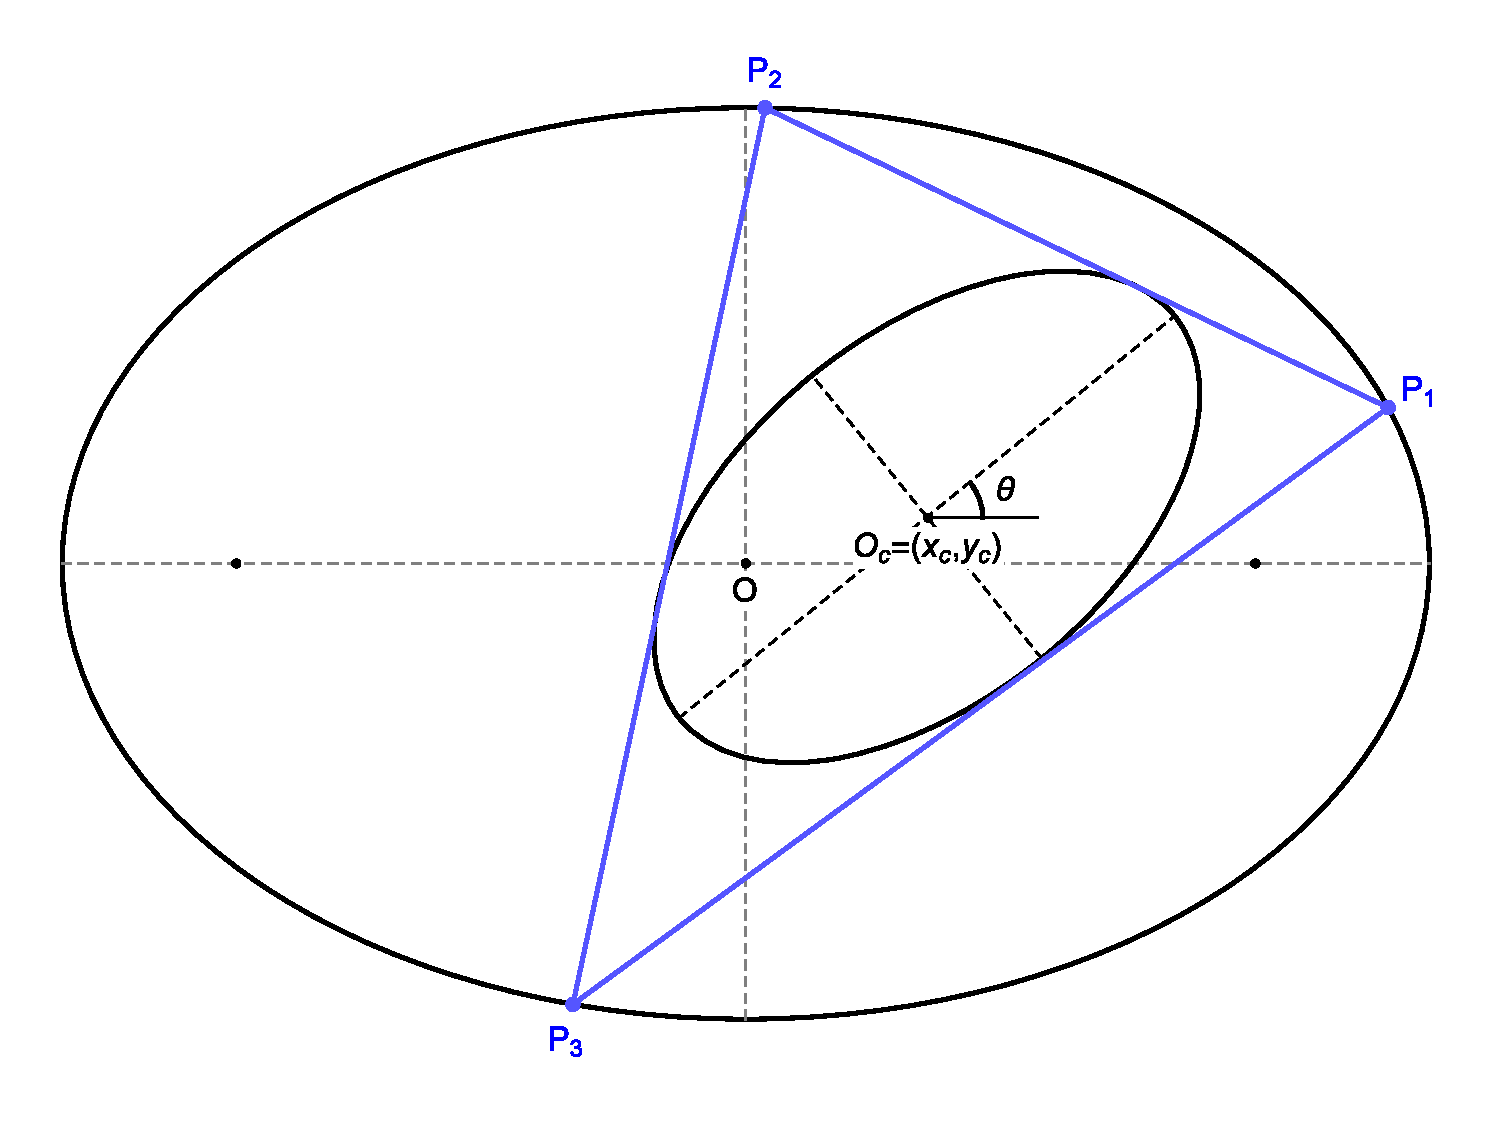
\includegraphics[width=.6\textwidth]{pics/0070_n3_nonconcentric.eps}
    \caption{A pair of ellipses in general position which admits a Poncelet 3-periodic family (blue). Let the outer one be centered at the origin $O$. Their major axes are tilted by $\theta$, and their centers displaced by $O_c=(x_c,y_c)$. \href{https://youtu.be/bjHpXVyXXVc}{Video}}
    \label{fig:n3-general-pos}
\end{figure}

\subsection*{Main Results}

\begin{itemize}
  \item Section~\ref{sec:axis-aligned}: We first show that over 3-periodics in several concentric, axis-aligned pairs -- confocal, homothetic, with incircle, with circumcircle, and excentral -- the power of the center with respect to either the circumcircle or Euler's circle is invariant. Using analytic geometry (with trilinear coordinates), we derive explicit formulas for said powers for each family.
  \item Section~\ref{sec:concentric-tilted}: using CAS-based manipulation, we generalize this by proving that the power of the center with respect to both Euler's circle and the circumcircle is invariant for 3-periodics for any generic concentric pair (aligned or not), Theorem~\ref{thm:power-concentric-unaligned}.
    \item Section~\ref{sec:nonconcentric-circumcircle}: We then consider 3-periodics in the non-concentric pair with circumcircle. Using  a special parametrization based on Blaschke products \cite{daepp-2019}, we show that loci of triangle centers which are fixed affine combinations of the barycenter and circumcenter are circles, whose centers are collinear along a line passing through the stationary circumcenter.
    \item Section~\ref{sec:nonconcentric-tilted} For the generic case of 3-periodics in the non-concentric, non-axis-aligned ellipse pair, we show that triangle centers which are fixed linear combinations of barycenter and circumcenter will trace out elliptic loci, Theorem~\ref{thm:ellipse-locus}. These include such centers as the orthocenter, the center of the Euler circle, the de Longchamps point, etc.; see Observation~\ref{obs:affine-euler-line}.
\end{itemize}

In Section~\ref{sec:open-questions} we conclude with a few experimental conjectures. Appendix~\ref{app:symbols} contains a list of symbols used herein.

\subsection*{Related Work}

In \cite{odehnal2011-poristic}, the loci of many triangle centers over the poristic family (fixed circumcenter and incenter) are shown to be either stationary, circular, or elliptic. In \cite{sergei2016-com}, the loci of vertex and area centroids are proved to be ellipses over a generic Poncelet family. The circumcenter of mass (which is simply the circumcenter for Poncelet 3-periodics) is shown to be an ellipse in \cite{sergei2014-circumcenter-of-mass}.
 
 Properties of 3-periodics in the confocal pair (elliptic billiard) were studied in \cite{reznik2020-intelligencer,garcia2020-new-properties}. A few results and their subsequent proofs include: the elliptic locus of the incenter \cite{olga14,garcia2019-incenter}, circumcenter \cite{garcia2019-incenter,corentin19}, invariant sum of cosines  \cite{akopyan2020-invariants,bialy2020-invariants}, and invariant ratio of outer-to-orbit polygon areas  \cite{caliz2020-area-product}. 
 
In \cite{garcia2020-ellipses} it was shown that over confocal 3-periodics, 29 triangle centers (out of the first 100 in \cite{etc}) trace out ellipses. Explicit expressions are given for the semi-axes of each locus. In subsequent works, we studied the relationship between (i) poristic triangles and the confocal family (poristic) \cite{garcia2020-similarity-I}, and (ii) the homothetic family and the Brocard porism \cite{reznik2020-similarityII}, showing that said pairs are images of each other under a variable similarity transform. In \cite{garcia2020-family-ties} we compare several loci and invariants across several concentric, axis-aligned pairs, grouping them into clusters.


 
